\documentclass[
	letterpaper, % Paper size, specify a4paper (A4) or letterpaper (US letter)
	10pt, % Default font size, specify 10pt, 11pt or 12pt
]{CSUniSchoolLabReport}

%----------------------------------------------------------------------------------------
%	REPORT INFORMATION
%----------------------------------------------------------------------------------------

\title{Dynamically Growing Arrays in C++\\ Embedded Design: Enabling Robotics \\ EECE2160} % Report title

\author{Michael \textsc{Brodskiy}\\ \small \href{mailto:Brodskiy.M@Northeastern.edu}{Brodskiy.M@Northeastern.edu}}

\date{March 23, 2023} % Date of the report

%----------------------------------------------------------------------------------------


\begin{document}

\maketitle % Insert the title, author and date using the information specified above

\begin{center}
	\begin{tabular}{l r}
		Date Performed: & March 16, 2023 \\ % Date the experiment was performed
        Partner: & Dylan \textsc{Powers} \\ % Partner names
		Instructor: & Professor \textsc{Shazli} % Instructor/supervisor
	\end{tabular}
\end{center}

\newpage

\begin{abstract}

  This laboratory experiment served as an introduction to pointers and array manipulation in \texttt{C++}. By having us generate logic to manipulate a value pointing to an array, we became more familiarized with pointer and array concepts.

\end{abstract}

\begin{flushleft}

  \textsc{Keywords:} \underline{\texttt{C++}}, \underline{array}, \underline{pointer}

\end{flushleft}

\newpage

\section{Equipment}

\hspace{.5 in} Available equipment included:\\

\begin{itemize}

  \item DE1-SoC board

  \item DE1-SoC Power Cable

  \item USB-A to USB-B Cable

  \item Computer

  \item MobaXTerm SSH Terminal

  \item USB-to-ethernet Adapter

\end{itemize}

\section{Introduction}

\hspace{.5 in} When creating a dynamically growing array, an initial region of memory is assigned to it. Then, as elements begin to be inserted into the array, the initial memory region is occupied, and, if necessary, expanded. In this lab, the goal was to serve as an introduction to implementing and modifying dynamically growing arrays into a program. To begin, a program was created to prompt a user to select an option from a menu of array modifications, shown below in Figure \ref{fig:1}:

\begin{figure}[H]
  \centering
  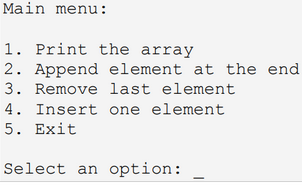
\includegraphics[width=.5\textwidth]{Figures/Menu.png}
  \caption{Menu of Array Modifications}
  \label{fig:1}
\end{figure}

\section{Discussion \& Analysis} 

\subsection{Assignment 1}

\hspace{.5 in} The goal of Assignment 1 was to write a program that displays the menu shown in Figure 1, and waits for a user to enter a selection. At this point, if a valid selection is made, the menu repeats except for the selection of  integer 5 where the program exits. However, If any user input was invalid, an error message displayed and the main menu repeated. Below is the output of an execution example where several different options were selected (Figures \ref{fig:2}-\ref{fig:3}).

\begin{figure}[H]
  \centering
  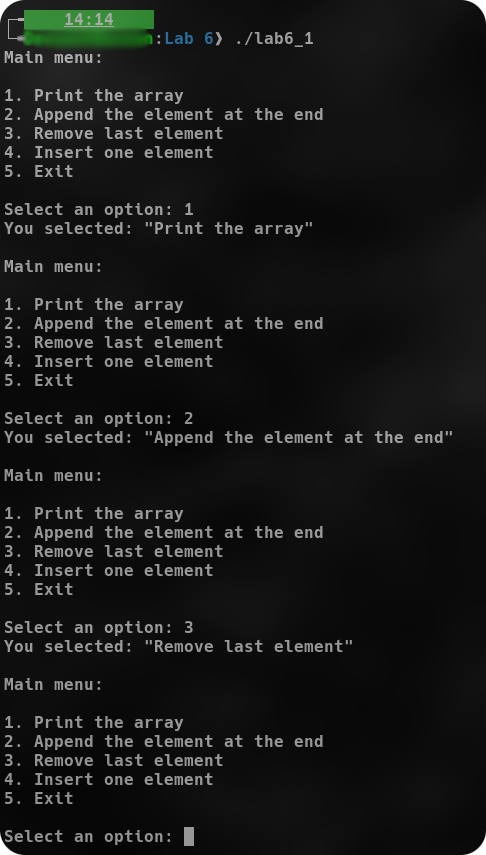
\includegraphics[height=.75\textheight]{Figures/6_1.png}
  \caption{Menu Selection Output}
  \label{fig:2}
\end{figure}

\begin{figure}[H]
  \centering
  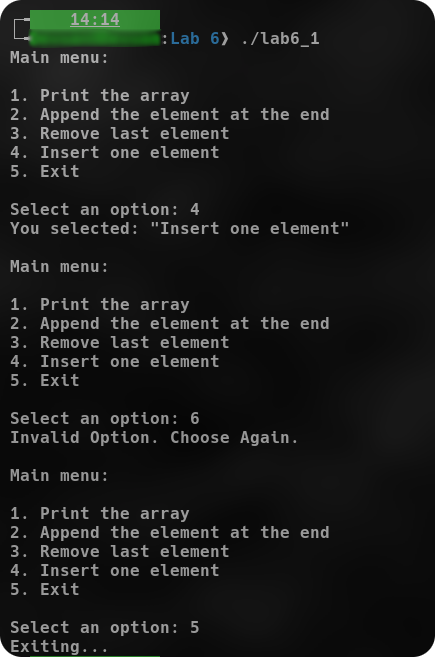
\includegraphics[height=.75\textheight]{Figures/6_1-2.png}
  \caption{Menu Selection Output 2}
  \label{fig:3}
\end{figure}

\subsection{Assignment 2}

\hspace{.5 in} The goal of Assignment 2 was to write a function \texttt{Grow()} that grows the capacity of the vector. The designed function increased the vector's allocated storage while keeping the same set of elements in the vector. The new code for the \texttt{Grow()} function is shown below in Listing \ref{lst:L1}. 

\newpage

\lstinputlisting[
    caption=\texttt{Grow()} Function Code, % Caption above the listing
    label=lst:L1, % Label for referencing this listing
    language=C++, % Use C++ functions/syntax highlighting
    frame=single, % Frame around the code listing
    showstringspaces=false, % Don't put marks in string spaces
    numbers=left, % Line numbers on left
    numberstyle=\tiny, % Line numbers styling
    backgroundcolor=\color{black!5}, % Set background color
    keywordstyle=\color{magenta!80}, % Set keyword color
    commentstyle=\color{blue!80}, % Set comment color
    stringstyle=\color{green!80}, % Set string color
    breaklines=true
  ]{Code/Grow.cpp}


\subsection{Assignment 3}

\hspace{.5 in} The goal of Assignment 3 was to write an \texttt{AddElement()} function capable of adding an element at the end of the vector even if the vector was full. This required invoking \texttt{Grow()} when the current number of present elements was equal to the capacity of the vector. Once it was ensured that there was enough storage capacity for a new element, the new element was safely added at the end of the vector. Along with \texttt{AddElement()}, a \texttt{PrintVector()} function was written to print the current elements contained within the vector. The code for both functions are shown below in Listings \ref{lst:L2} and \ref{lst:L3}. 

\lstinputlisting[
    caption=\texttt{AddElement()} Function Code, % Caption above the listing
    label=lst:L2, % Label for referencing this listing
    language=C++, % Use C++ functions/syntax highlighting
    frame=single, % Frame around the code listing
    showstringspaces=false, % Don't put marks in string spaces
    numbers=left, % Line numbers on left
    numberstyle=\tiny, % Line numbers styling
    backgroundcolor=\color{black!5}, % Set background color
    keywordstyle=\color{magenta!80}, % Set keyword color
    commentstyle=\color{blue!80}, % Set comment color
    stringstyle=\color{green!80}, % Set string color
    breaklines=true
  ]{Code/AddElement.cpp}

\lstinputlisting[
    caption=\texttt{PrintVector()} Function Code, % Caption above the listing
    label=lst:L3, % Label for referencing this listing
    language=C++, % Use C++ functions/syntax highlighting
    frame=single, % Frame around the code listing
    showstringspaces=false, % Don't put marks in string spaces
    numbers=left, % Line numbers on left
    numberstyle=\tiny, % Line numbers styling
    backgroundcolor=\color{black!5}, % Set background color
    keywordstyle=\color{magenta!80}, % Set keyword color
    commentstyle=\color{blue!80}, % Set comment color
    stringstyle=\color{green!80}, % Set string color
    breaklines=true
  ]{Code/PrintVector.cpp}

  Additionally, the output of the program for an execution where several elements were added to a vector and the current content of the vector was printed is shown in Figures \ref{fig:4}-\ref{fig:5}.

  \begin{figure}[H]
    \centering
    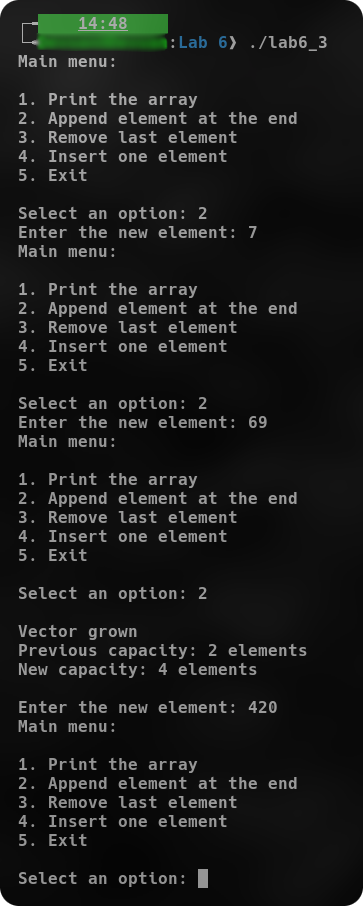
\includegraphics[height=.9\textheight]{Figures/6_3.png}
    \caption{Assignment 3 Execution}
    \label{fig:4}
  \end{figure}

  \begin{figure}[H]
    \centering
    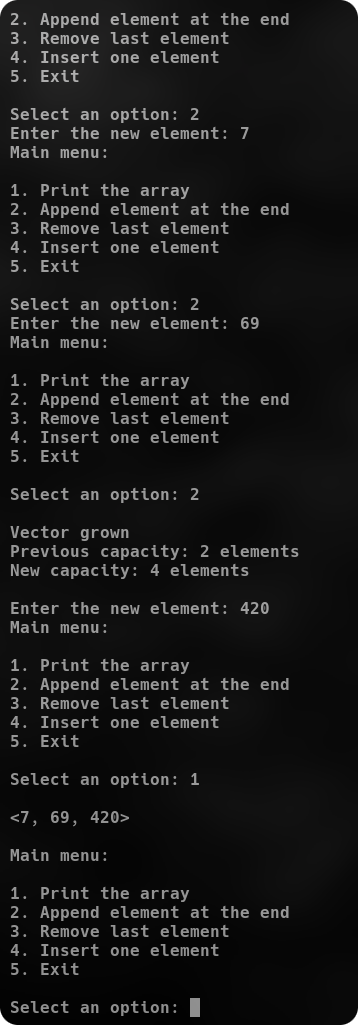
\includegraphics[height=.8\textheight]{Figures/6_3-2.png}
    \caption{Assignment 3 Execution Part 2}
    \label{fig:5}
  \end{figure}

  \subsection{Assignment 4} \hspace{.5 in} The goal of Assignment 4 was to write a \texttt{RemoveElement()} function accessible through option 3 in the main menu that removed the last element contained in the vector. Additionally, the program displayed a proper error message indicating that there are no elements in the vector to remove when the vector was empty and the user selected option 3. The code for the \texttt{RemoveElement()} function is shown in Listing \ref{lst:L4}. 

\lstinputlisting[
    caption=\texttt{RemoveElement()} Function Code, % Caption above the listing
    label=lst:L4, % Label for referencing this listing
    language=C++, % Use C++ functions/syntax highlighting
    frame=single, % Frame around the code listing
    showstringspaces=false, % Don't put marks in string spaces
    numbers=left, % Line numbers on left
    numberstyle=\tiny, % Line numbers styling
    backgroundcolor=\color{black!5}, % Set background color
    keywordstyle=\color{magenta!80}, % Set keyword color
    commentstyle=\color{blue!80}, % Set comment color
    stringstyle=\color{green!80}, % Set string color
    breaklines=true
  ]{Code/RemoveElement.cpp}

  An output of the program removing the last element successfully and an output where the function is invoked on an empty vector are shown in Figures \ref{fig:6}-\ref{fig:8}. 

  \begin{figure}[H]
    \centering
    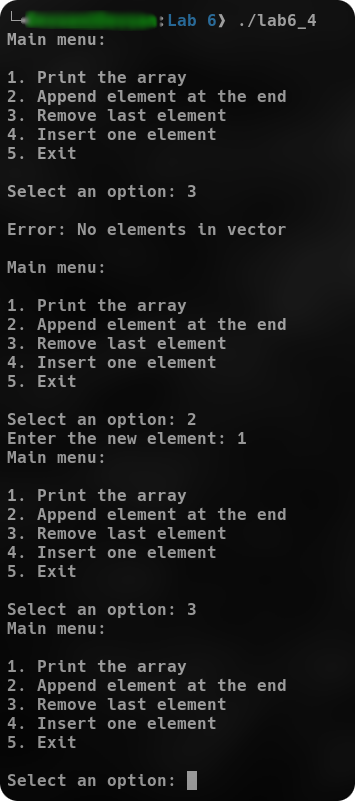
\includegraphics[height=.9\textheight]{Figures/6_4.png}
    \caption{Assignment 4 Execution}
    \label{fig:6}
  \end{figure}

  \begin{figure}[H]
    \centering
    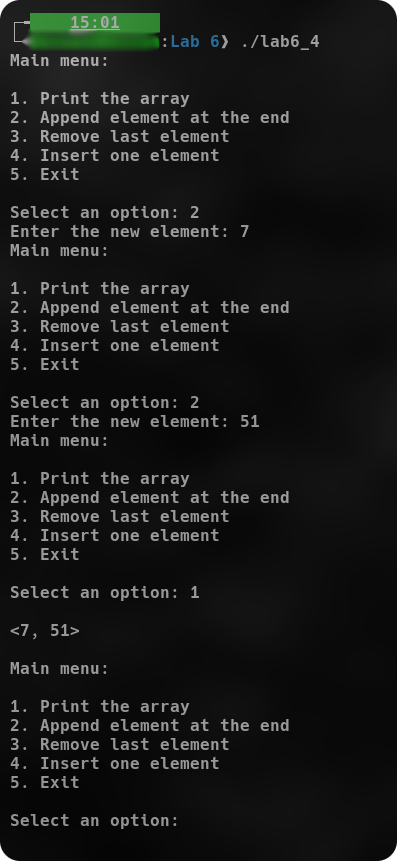
\includegraphics[height=.9\textheight]{Figures/6_4-2.png}
    \caption{Assignment 4 Execution Part 2}
    \label{fig:7}
  \end{figure}

  \begin{figure}[H]
    \centering
    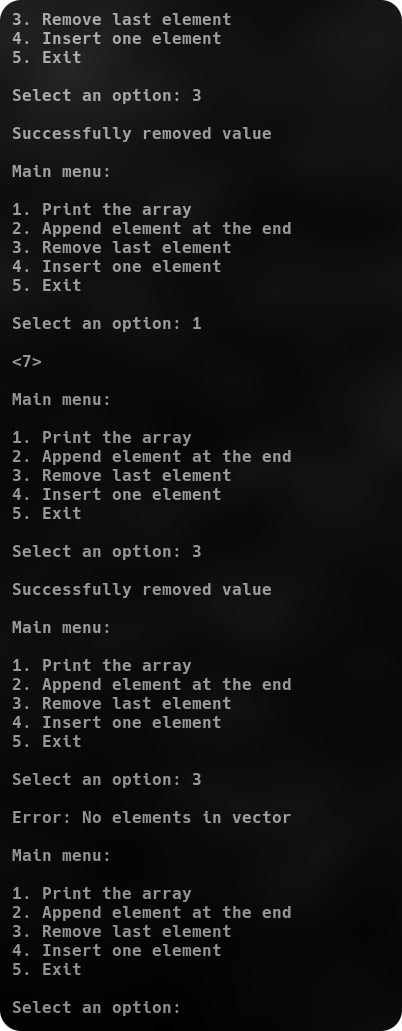
\includegraphics[height=.7\textheight]{Figures/6_4-3.png}
    \caption{Assignment 4 Execution Part 3}
    \label{fig:8}
  \end{figure}

  \subsection{Assignment 5} \hspace{.5 in} The goal of Assignment 5 was to write an \texttt{InsertElement()} function and have it accessible to the user through option 4 in the menu. The function asks the user for an index and a value for the new element. The index is then checked for correct boundaries, and a proper error message is displayed if the entered value is invalid. The code for \texttt{InsertElement()} is shown below in Listing \ref{lst:L5}.

\lstinputlisting[
    caption=\texttt{InsertElement()} Function Code, % Caption above the listing
    label=lst:L5, % Label for referencing this listing
    language=C++, % Use C++ functions/syntax highlighting
    frame=single, % Frame around the code listing
    showstringspaces=false, % Don't put marks in string spaces
    numbers=left, % Line numbers on left
    numberstyle=\tiny, % Line numbers styling
    backgroundcolor=\color{black!5}, % Set background color
    keywordstyle=\color{magenta!80}, % Set keyword color
    commentstyle=\color{blue!80}, % Set comment color
    stringstyle=\color{green!80}, % Set string color
    breaklines=true
  ]{Code/InsertElement.cpp}

Screenshots for testing the overall code are shown below in Figures \ref{fig:9}-\ref{fig:10}.

\begin{figure}[H]
  \centering
  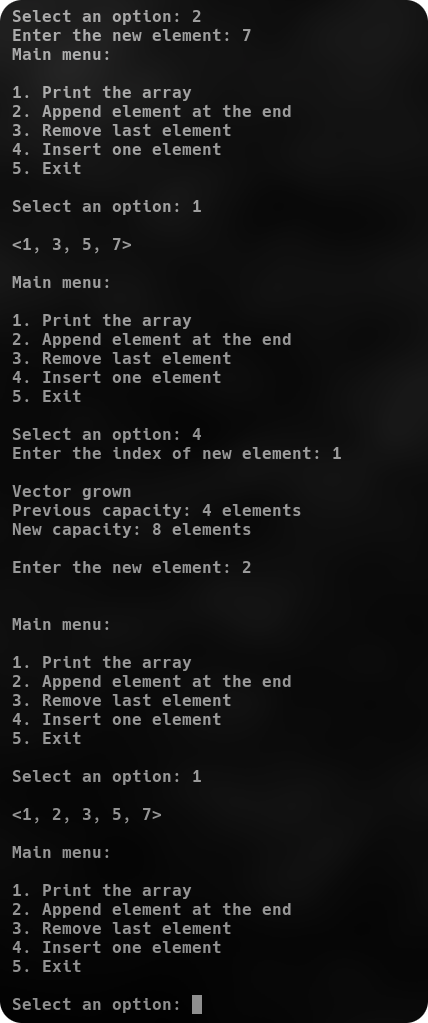
\includegraphics[height=.9\textheight]{Figures/6_4-4.png}
  \caption{Code Testing}
  \label{fig:9}
\end{figure}

\begin{figure}[H]
  \centering
  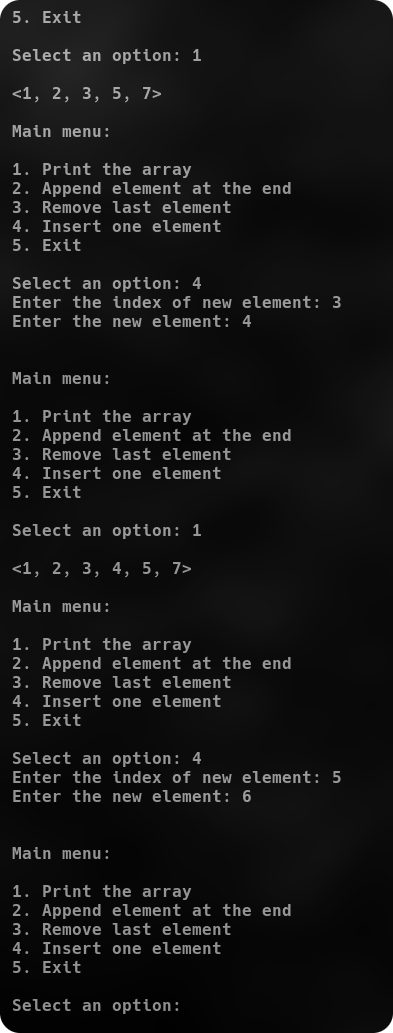
\includegraphics[height=.75\textheight]{Figures/6_4-5.png}
  \caption{Code Testing Part 2}
  \label{fig:10}
\end{figure}

\section{Conclusion}

\hspace{.5 in} Overall, this lab resulted in the creation of a menu-modified, dynamically-grown array. Through memory allocation and expansion, in tandem with element addition, insertion, and removal logic, the aforementioned dynamically-growing array was constructed. As such, this laboratory experiment demonstrated memory allocation concepts in \texttt{C++}.

\section{Appendix}

\lstinputlisting[
    caption=Complete Source Code, % Caption above the listing
    label=lst:L6, % Label for referencing this listing
    language=C++, % Use C++ functions/syntax highlighting
    frame=single, % Frame around the code listing
    showstringspaces=false, % Don't put marks in string spaces
    numbers=left, % Line numbers on left
    numberstyle=\tiny, % Line numbers styling
    backgroundcolor=\color{black!5}, % Set background color
    keywordstyle=\color{magenta!80}, % Set keyword color
    commentstyle=\color{blue!80}, % Set comment color
    stringstyle=\color{green!80}, % Set string color
    breaklines=true
  ]{Code/lab6_5.cpp}

\end{document}
